%% KSAE 2-column format paper
%% Modified from Elsevier template to 2-column layout
\documentclass[final,5p,times,twocolumn,9pt]{elsarticle}
%% Note: Using 5p option for 2-column format with 9.5pt font
%% The amssymb package provides various useful mathematical symbols
\usepackage{amssymb}
%% The amsmath package provides various useful equation environments.
\usepackage{amsmath}
%% Korean language support
\usepackage{kotex}
\usepackage[utf8]{inputenc}
\usepackage{CJKutf8}
%% KSAE margin settings
\usepackage{geometry}
\geometry{
left=2.1cm, right=3.4cm, top=2.6cm, bottom=2.5cm }
%% Line spacing adjustment - Fixed 14pt as in Word
\usepackage{setspace}
\setlength{\baselineskip}{14pt}
%% Additional packages
\usepackage{siunitx}    % For units and scientific notation
\usepackage{url}        % For URLs
\usepackage[dvipsnames]{xcolor} % For colored text
\usepackage{subfigure}   % For subfigures
\usepackage{listings}    % For code listings
\usepackage{algorithm}
\usepackage{algorithmic}
\usepackage[most]{tcolorbox}  % For LLM response boxes

%% Custom macros for code variables (prevents overfull hbox)
\newcommand{\code}[1]{\texttt{\mbox{#1}}}

%% LLM response box styles
\newtcolorbox{llmbox}[1][]{
colback=gray!5, colframe=gray!60, fonttitle=\bfseries\small, title={#1}, boxrule=0.5pt, arc=2pt, left=4pt, right=4pt, top=2pt, bottom=2pt, fontupper=\small }

%% Code listing style for command format
\lstset{
basicstyle=\ttfamily\small, breaklines=true, frame=single, backgroundcolor=\color{gray!10}, columns=fullflexible }

%% Graphics path for figures
\graphicspath{{figures/}}


\journal{KSAE}

\begin{document}

\begin{frontmatter}

%% Title, authors and addresses

\title{LLM 에이전트를 활용한 CarMaker 기반 자율주행 시뮬레이션 의사결정 시스템}


\author[1]{Kyoungtae Ji}
\author[1]{Dongyeol Won}
\author[1]{Chanhyeok Ko}
\author[1]{Kyoungseok Han\corref{cor1}}
\ead{kyoungsh@hanyang.ac.kr}
\cortext[cor1]{Corresponding author}

\affiliation[1]{organization={Department of Automotive Engineering, Hanyang University},
country={South Korea}}

\begin{abstract}
This study proposes an autonomous driving decision-making system for CarMaker simulation using a large language model (LLM) agent. Conventional rule-based and reinforcement learning approaches to autonomous driving decision-making have limitations in scenario scalability and generalization. We design a trigger-based control loop that pauses the simulation when the vehicle state meets a predefined condition, requests a driving decision from the LLM, and sequentially executes the generated control commands. To this end, we define a unified command format that converts LLM outputs into vehicle control inputs and develop a dynamic prompt system that flexibly configures decision strategies for different scenarios. In a CarMaker simulation of an urban pedestrian emergency avoidance scenario, three control methods---Rule-based, LLM Single-shot, and LLM Feedback Loop---are compared. The results demonstrate that the Feedback Loop approach enables the LLM to autonomously analyze the causes of previous decision failures and correct control parameters, suggesting the potential for self-correction in LLM-based vehicle control.
\end{abstract}


%% Keywords
\begin{keyword}
Large language model(대규모 언어모델) \sep Autonomous driving(자율주행) \sep Decision making(의사결정) \sep Driving simulation(주행 시뮬레이션) \sep CarMaker \sep Trigger-based control(트리거 기반 제어)
\end{keyword}

\end{frontmatter}


%% ============================================================
%% SECTION 1: INTRODUCTION (~0.7p)
%% ============================================================
\section{서론}
\label{sec:introduction}

자율주행 차량의 의사결정은 주변 환경을 인식하고 안전하고 효율적인 주행 전략을 수립하는 핵심 과제이다. 기존의 규칙 기반(rule-based) 접근법은 유한 상태 기계(FSM)나 의사결정 트리를 활용하여 명확한 판단 로직을 제공하지만, 복잡한 도심 환경이나 예상치 못한 엣지 케이스에 대한 확장성이 부족하다는 한계가 있다. 강화학습(reinforcement learning) 기반 방법은 시뮬레이션 환경에서 최적 정책을 학습할 수 있으나, 보상 함수 설계의 어려움, 긴 학습 시간, 그리고 학습되지 않은 시나리오에 대한 일반화 한계가 존재한다\cite{pang2026large, ryu2025curricullm}.

최근 대규모 언어모델(Large Language Model, LLM)의 급격한 발전은 자율주행 연구에 새로운 패러다임을 제시하고 있다. LLM은 방대한 텍스트 데이터로부터 학습한 추론 능력을 바탕으로 복잡한 상황을 자연어로 이해하고 판단할 수 있으며, 프롬프트 변경만으로 행동 전략을 조정할 수 있어 재학습이 불필요하다는 장점이 있다. Mao et al.\cite{mao2023gpt}은 GPT-3.5를 motion planner로 활용하여 궤적 좌표를 언어 토큰으로 생성하는 접근법을 제안하였으며, Lu et al.\cite{lu2025omnitester}은 LLM과 VLM을 결합하여 엣지 케이스 시나리오를 자동 생성하는 프레임워크를 제시하였다. 또한 LLM을 강화학습의 가이드로 활용하여 보상 함수를 자동 설계하거나 학습 커리큘럼을 조정하는 연구도 활발히 진행되고 있다\cite{liang2024eurekaverse, pang2026large, ryu2025curricullm}.

한편, LLM을 자율주행의 직접적인 의사결정 주체로 활용하려는 연구도 등장하고 있다. Wen et al.\cite{wen2023dilu}은 LLM에 추론 및 반성 모듈을 두어 경험을 축적하는 지식 기반 자율주행 프레임워크를 제안하였으며, Fu et al.\cite{fu2024drive}은 LLM의 추론, 해석, 기억 능력을 장기 미경험(long-tail) 시나리오 대응에 활용할 수 있음을 보였다.

또한 LLM 분야에서는 Reflexion\cite{shinn2023reflexion}이나 Self-Refine\cite{madaan2023self}과 같이 LLM이 자신의 출력을 반복적으로 평가하고 개선하는 자기 보정(self-correction) 메커니즘이 보고되어 있으나, 이를 차량 제어 도메인에 적용한 연구는 아직 이루어지지 않았다. 기존 연구들은 주로 오프라인 계획 수립이나 강화학습 보조에 초점을 두며, 시뮬레이션 환경에서 LLM이 차량 상태를 판단하고 직접 제어 명령을 생성하는 온라인 의사결정 구조에 대한 연구는 부족하다. 본 연구는 이러한 한계를 해결하기 위해 LLM 에이전트 기반의 CarMaker 자율주행 시뮬레이션 의사결정 시스템을 제안한다.

본 연구의 주요 기여는 다음과 같다:
\begin{itemize}
\item 차량 텔레메트리를 온라인으로 모니터링하고 조건 충족 시 시뮬레이션을 일시정지하여 LLM에 판단을 요청하는 트리거 기반 제어 루프를 설계하였다.
\item LLM의 자연어 출력을 CarMaker 차량 제어 입력으로 변환하는 통합 명령 포맷을 정의하였다.
\item 대화 이력 기반 피드백 루프를 통해 LLM이 이전 판단 결과를 반영하고 점진적으로 제어를 개선하는 반복적 의사결정 구조를 제안하였다.
\end{itemize}


%% ============================================================
%% SECTION 2: SYSTEM ARCHITECTURE (~1.5p)
%% ============================================================
\section{시스템 아키텍처}
\label{sec:architecture}

\subsection{전체 시스템 개요}
\label{sec:system_overview}

\begin{figure*}[!htbp]
	\centering
	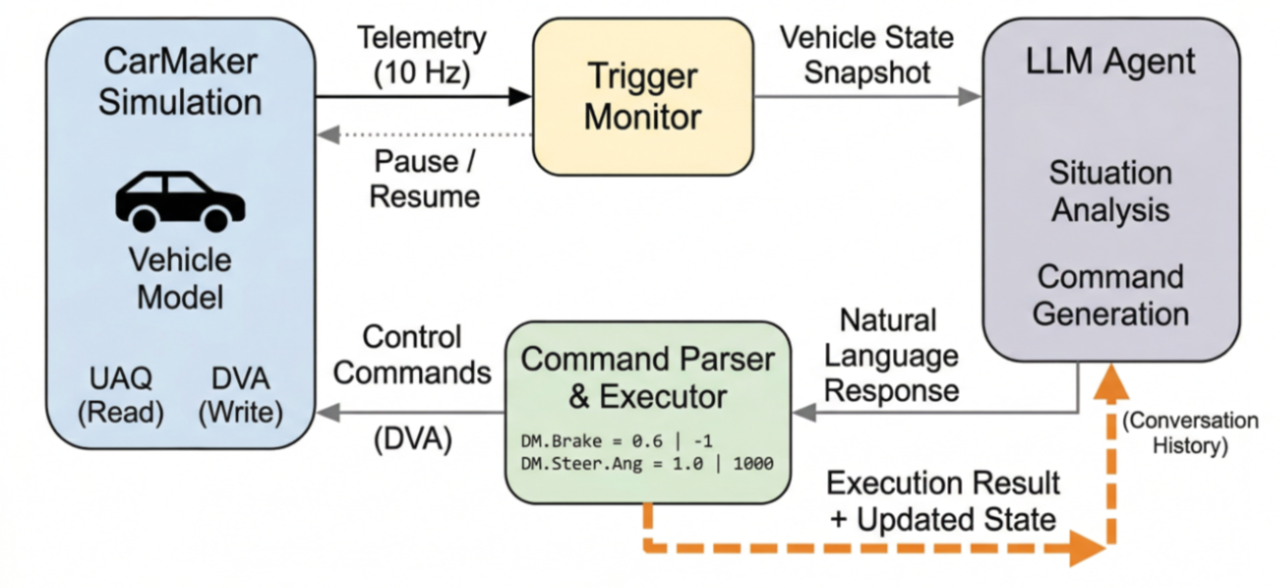
\includegraphics[width=\textwidth]{Overview2.png}
	\caption{LLM 에이전트 기반 자율주행 판단 시스템의 전체 아키텍처. 대화 인터페이스와 트리거 모니터가 CarMaker 시뮬레이션 및 LLM과 연동되어 시뮬레이션 연동형 판단과 제어를 수행한다.}
	\label{fig_system_architecture}
\end{figure*}

제안하는 시스템은 Figure~\ref{fig_system_architecture}에 나타낸 바와 같이 CarMaker 시뮬레이션, 트리거 모니터, LLM 에이전트, 명령 실행기의 네 가지 핵심 모듈로 구성된다. CarMaker와는 TCP 소켓을 통해 실시간으로 통신하며, LLM은 별도 프로세스를 통해 추론을 수행한다.

데이터 흐름은 다음과 같다: CarMaker 시뮬레이션에서 10\,Hz 주기로 차량 텔레메트리(속도, 가속도, 조향각 등)를 수집하고, 트리거 모니터가 사전 정의된 조건을 평가한다. 조건이 충족되면 시뮬레이션을 일시정지(time scale $\rightarrow$ 0.001$\times$)한 후 차량 상태 스냅샷을 LLM에 전달하여 판단을 요청한다. LLM이 생성한 응답은 명령 파서에 의해 구조화된 제어 명령으로 변환되고, 명령 실행기가 이를 CarMaker에 순차적으로 전달한 뒤 시뮬레이션을 재개(time scale $\rightarrow$ 1.0$\times$)한다.


\subsection{CarMaker TCP 실시간 통신}
\label{sec:carmaker_tcp}


본 시스템과 CarMaker 간의 통신은 CarMaker에 내장된 Tcl 스크립트 인터페이스를 통해 이루어진다.

CarMaker는 UAQ(User Accessible Quantities)와 DVA(Direct Variable Access)를 통해 시뮬레이션 내부 신호에 대한 양방향 접근을 제공한다. UAQ는 차량 속도, 종가속도, 요 레이트 등 CarMaker가 사전 정의한 차량 상태 변수를 실시간으로 읽을 수 있는 인터페이스이며, DVA는 Driver Model의 가속, 제동, 조향 등 제어 신호에 직접 값을 쓸 수 있는 메커니즘이다.

본 시스템은 TCP 소켓을 통해 이러한 신호에 접근한다. 트리거 모니터는 UAQ를 통해 차량 상태를 10\,Hz 주기로 수신하여 트리거 조건을 평가하고, LLM이 생성한 제어 명령은 DVA를 통해 CarMaker의 Driver Model에 실시간으로 반영된다. 이러한 양방향 통신 구조를 통해 시뮬레이션 상태의 온라인 모니터링과 LLM 기반 제어 명령의 즉시 반영이 가능하다.


\subsection{트리거 기반 제어 루프}
\label{sec:trigger_loop}

\begin{figure}[tbp!]
	\centering
	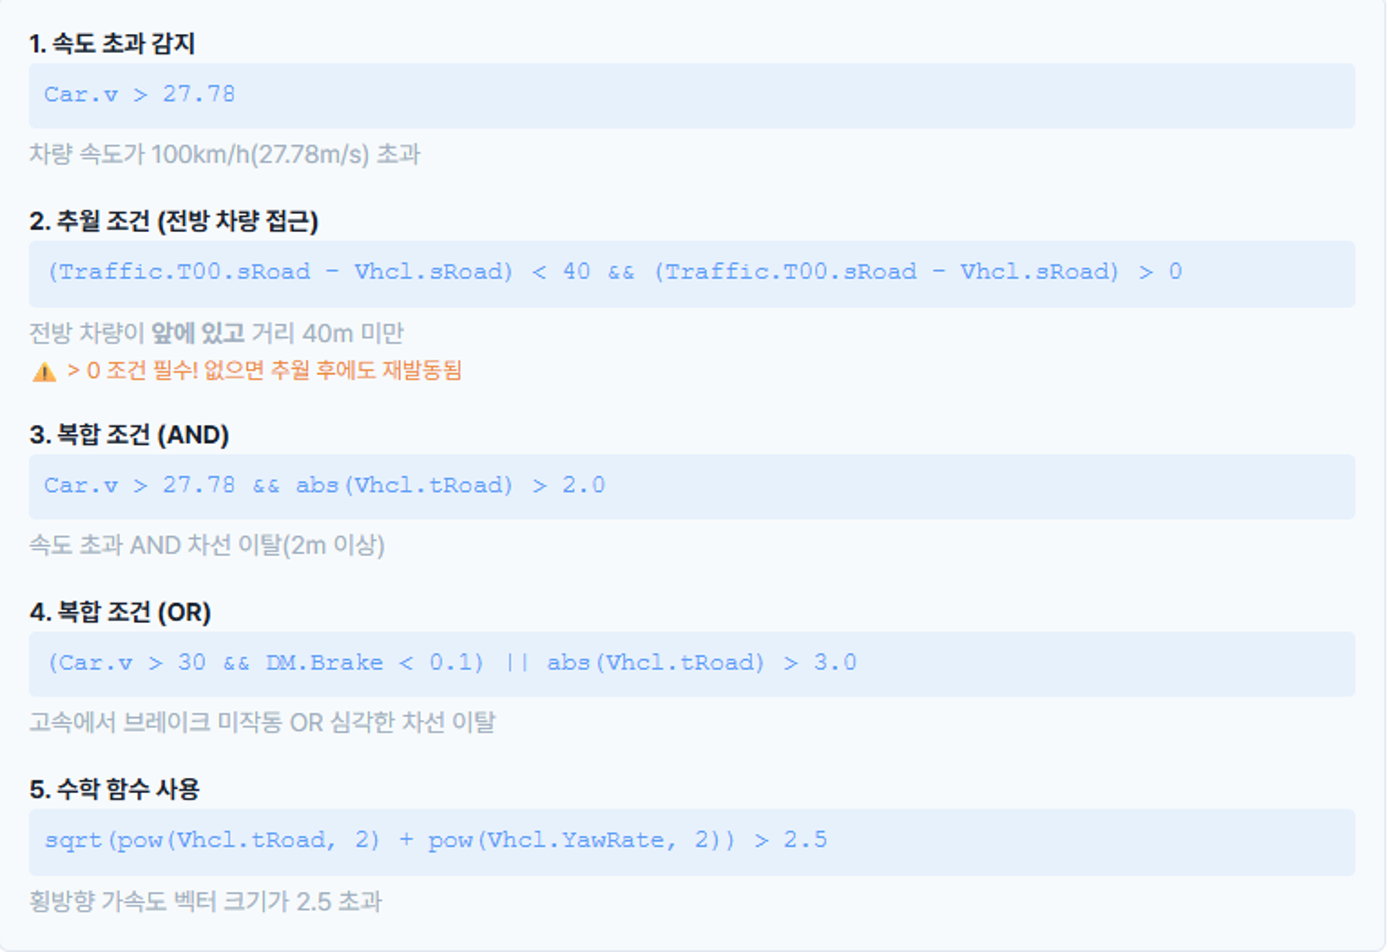
\includegraphics[width=\columnwidth]{Trigger_Examples.png}
	\caption{트리거 조건 설정 예시. 속도 초과, 추돌 조건, 복합 조건(AND/OR), 수학 함수 활용 등 다양한 형태의 트리거를 사용자가 정의할 수 있다.}
	\label{fig_trigger_examples}
\end{figure}

트리거 기반 제어 루프는 본 시스템의 핵심 메커니즘으로, LLM의 응답 지연 문제를 시뮬레이션 일시정지를 통해 해결한다. Figure~\ref{fig_trigger_examples}는 사용자가 정의할 수 있는 다양한 트리거 조건의 예시를 나타낸다.

트리거는 사용자가 정의한 조건식으로 구성되며, 차량 상태 변수에 대한 비교 연산을 지원한다. 예를 들어, 차량 속도가 100\,km/h 이상이거나 종가속도가 $-5.0$\,m/s$^2$ 미만인 급감속 상황에서 트리거가 발동한다.

트리거 발동 시 시스템은 다음 순서로 동작한다: (1) 시뮬레이션 시간 스케일을 0.001$\times$로 설정하여 사실상 정지시킨다. (2) 현재 차량 상태(속도, 가속도, 조향각, 위치 등)를 스냅샷으로 캡처한다. (3) 스냅샷과 함께 구성된 프롬프트를 LLM에 전달한다. (4) LLM 응답을 파싱하여 제어 명령 시퀀스를 추출한다. (5) 시뮬레이션을 재개(time scale $\rightarrow$ 1.0$\times$)하고 명령을 순차 실행한다. (6) 5초간의 쿨다운 기간을 두어 동일 트리거의 중복 발동을 방지한다.

이 구조는 LLM의 추론 시간(수 초)이 시뮬레이션 시간에 영향을 미치지 않도록 하면서도, 온라인 차량 상태에 기반한 동적 의사결정을 가능하게 한다.


\subsection{통합 명령 포맷}
\label{sec:command_format}

LLM이 생성하는 자연어 응답을 CarMaker의 차량 제어 입력으로 변환하기 위해, 본 연구에서는 다음과 같은 통합 명령 포맷을 설계하였다:

\begin{lstlisting}
DM.Gas = <value> | <duration_ms>
DM.Brake = <value> | <duration_ms>
DM.Steer.Ang = <value> | <duration_ms>
wait <milliseconds>
wait_until <condition>
\end{lstlisting}

각 명령은 제어 변수, 목표값, 지속 시간(밀리초)으로 구성되며, 모든 명령은 위에서 아래로 순차적으로 실행된다. wait 명령은 명시적 지연을 삽입하고, wait\_until 명령은 차량 상태가 특정 조건을 만족할 때까지 대기한다.

이 포맷의 설계 원칙은 다음 세 가지이다: (1) LLM이 생성하기 쉬운 단순한 텍스트 형식, (2) CarMaker의 다양한 제어 모드를 내부적으로 추상화, (3) 순차 실행과 조건부 대기를 통한 복합 기동 표현.

예를 들어, 긴급 제동 시나리오에서 LLM은 다음과 같은 명령 시퀀스를 생성한다:

\begin{lstlisting}
DM.Gas = 0.0 | 500
DM.Brake = 0.8 | 3000
wait_until Car.v <= 3.0
DM.Brake = 0.0 | 500
\end{lstlisting}

이는 가속 페달을 해제(500\,ms)한 후 80\% 제동을 가하고(3000\,ms), 차량 속도가 3.0\,m/s 이하가 될 때까지 대기한 뒤 제동을 해제하는 동작을 의미한다. 모든 제어 명령은 내부적으로 절대값 모드로 처리되어, LLM이 제어 모드를 별도로 지정하지 않아도 예측 가능한 차량 거동을 보장한다.


%% ============================================================
%% SECTION 3: EXPERIMENTAL SETUP (~1.5p)
%% ============================================================
\section{실험 환경 및 방법}
\label{sec:methodology}

\subsection{시뮬레이션 환경}
\label{sec:simulation_env}

\begin{figure}[tbp!]
	\centering
	\subfigure[Rule-based (AEB 제동만 적용)]{
		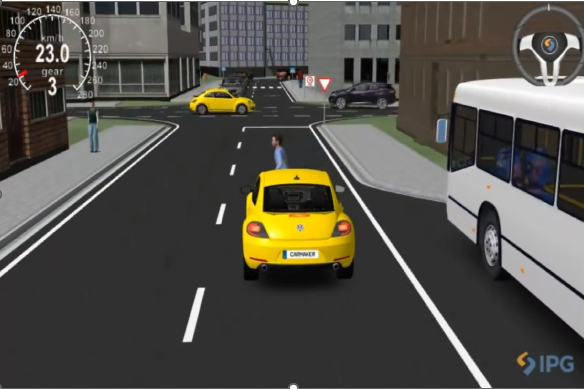
\includegraphics[width=0.95\columnwidth]{Video_LLM_none.png}
		\label{fig_result_none}
	}
	\subfigure[LLM Single-shot (1회 판단)]{
		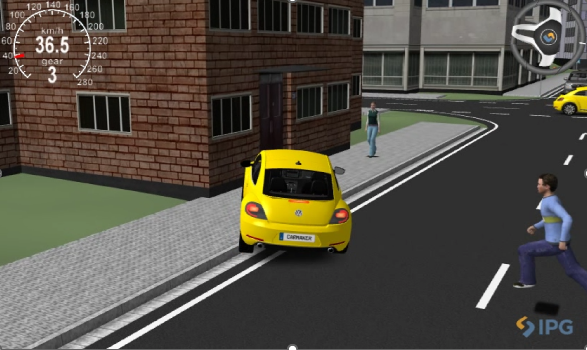
\includegraphics[width=0.95\columnwidth]{Video_LLM_Single.png}
		\label{fig_result_single}
	}
	\subfigure[LLM Feedback Loop (반복 판단)]{
		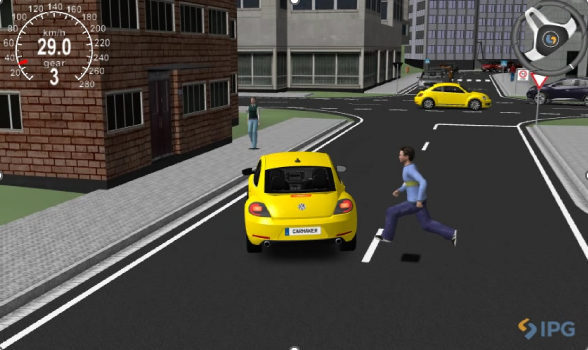
\includegraphics[width=0.95\columnwidth]{Video_LLM_loop.png}
		\label{fig_result_loop}
	}
	\caption{CarMaker AEB 테스트 시나리오에서의 제어 방식별 차량 거동 비교. (a) Rule-based: 제동만으로 보행자 충돌 불가피, (b) Single-shot: 좌측 회피를 시도하나 과조향으로 건물과 충돌, (c) Feedback Loop: 이전 판단을 보정하여 보행자 회피 및 차로 내 제어 유지.}
	\label{fig_scenario_comparison}
\end{figure}

실험은 IPG CarMaker를 사용하여 수행하였다. Section~\ref{sec:carmaker_tcp}에서 기술한 바와 같이 TCP 소켓과 UAQ/DVA 인터페이스를 통해 10\,Hz 주기로 차량 상태를 수신하고, 제어 명령과 시뮬레이션 시간 스케일을 실시간으로 제어한다.

LLM은 Anthropic Claude Sonnet 4.6을 사용하며, 프롬프트와 차량 상태 데이터를 텍스트 형태로 전달하고 응답을 통합 명령 포맷으로 변환하여 실행한다. LLM에 전달되는 프롬프트는 트리거 발동 시점의 차량 상태 스냅샷(Vehicle State)과 이전 판단 이력(Conversation History)을 포함한다. 특히 Conversation History는 Feedback Loop 방식에서 핵심적인 역할을 하며, 이전 판단에서 생성한 제어 명령과 그 실행 결과를 누적적으로 LLM에 전달함으로써 상황 변화에 적응적인 반복 판단을 가능하게 한다.


\subsection{평가 시나리오 및 지표}
\label{sec:evaluation}

제안 시스템의 성능을 검증하기 위해 도심 무단횡단 보행자 긴급 회피 시나리오를 설계하였다. 본 시나리오는 CarMaker에서 제공하는 AEB(Autonomous Emergency Braking) 테스트 시나리오를 기반으로 한다. 시험 차량이 도심 도로를 주행하며 정차된 버스에 접근하는 과정에서, 버스 뒤편의 사각지대로부터 보행자가 갑작스럽게 무단횡단하는 상황이다. 기존 AEB 테스트 시나리오 대비 차량 속도를 약 65\,km/h로 상향 조정하여, 일반적인 AEB 제동만으로는 충돌 회피가 어려운 조건을 구성하였다. 김동균 등\cite{kim2020collision}이 분석한 바와 같이 제동만으로 회피가 불가능한 상황에서는 조향을 포함한 복합 판단이 필수적이며, 본 시나리오는 이러한 고난이도 회피 상황에서의 LLM 판단 능력을 평가한다.

이 시나리오에 대해 다음 세 가지 제어 방식의 판단 품질을 비교한다:

\begin{itemize}
\item \textbf{Rule-based}: 사전 정의된 규칙에 따른 고정 제동 명령 실행
\item \textbf{LLM Single-shot}: 트리거 발동 시 LLM에 1회 판단을 요청하여 명령 생성
\item \textbf{LLM Feedback Loop}: LLM 판단 후 명령을 실행하고, 변화된 차량 상태를 다시 LLM에 전달하여 추가 판단을 반복하는 피드백 루프 방식
\end{itemize}

특히 Feedback Loop 방식은 이전 판단 결과와 현재 차량 상태를 대화 이력으로 누적 전달함으로써 상황 변화에 적응적인 판단을 가능하게 한다.


%% ============================================================
%% SECTION 4: RESULTS (~1.5p)
%% ============================================================
\section{실험 결과}
\label{sec:results}

도심 무단횡단 보행자 긴급 회피 시나리오에서 세 가지 제어 방식(Rule-based, LLM Single-shot, LLM Feedback Loop)의 성능을 비교하였다. 시험 차량은 약 65\,km/h(18.1\,m/s)로 주행 중이며, 정차된 버스 뒤편 사각지대에서 보행자가 출현하여 AEB 트리거가 발동한다. 일반 AEB 제동만으로는 충돌 회피가 불가능한 조건에서 각 방식이 제동과 조향을 어떻게 판단하는지를 비교하였다. Figure~\ref{fig_scenario_comparison}는 세 가지 제어 방식의 시뮬레이션 장면을, Figure~\ref{fig_trajectory}는 차량 궤적을, Figure~\ref{fig_control}과 Figure~\ref{fig_response}는 제어 입력 및 차량 응답의 시계열 비교를 나타낸다.

LLM Single-shot 방식에서 LLM은 1회 판단으로 다음과 같은 응답을 생성하였다:

\begin{llmbox}[LLM 응답 --- Single-shot (1차 판단)]
\textbf{상황 분석}: 긴급 충돌 회피 상황. 보행자가 갑자기 나타났으며, AEB 시스템이 활성화되어 있음. 현재 차량 속도는 약 65\,km/h (18.1\,m/s). 즉시 제동과 조향을 통해 보행자를 회피해야 함.

\textbf{제어 명령}:
\begin{lstlisting}
DM.Brake = 0.5 | -1
DM.Steer.Ang = 1.4 | 1000
wait_until Car.v <= 0.5
\end{lstlisting}
\end{llmbox}

\noindent LLM은 제동력 0.5와 조향각 1.4\,rad의 복합 회피 기동을 지시하였으나, 과도한 조향으로 인해 차량이 좌측 보도 영역까지 이탈하여 구조물과 충돌하였다.

LLM Feedback Loop 방식에서는 1차 판단의 실행 결과(좌측 이탈 및 충돌)가 대화 이력으로 LLM에 재전달되었으며, LLM은 2차 판단에서 이전 시도의 문제점을 자체적으로 분석하고 제어 파라미터를 보정하였다:

\begin{llmbox}[LLM 응답 --- Feedback Loop (2차 판단)]
\textbf{상황 분석}: 이전 회피 시도에서 조향각이 너무 컸고(1.4\,rad), 차량이 왼쪽으로 과도하게 이탈하여 건물과 충돌했음. 현재 속도 약 64\,km/h (17.78\,m/s), AEB 활성화 상태. 이번에는 조향각을 줄이고 제동력을 높여 제어된 회피 기동을 수행.

\textbf{제어 명령}:
\begin{lstlisting}
DM.Brake = 0.6 | -1
DM.Steer.Ang = 1.0 | 1000
wait_until Car.v <= 0.5
\end{lstlisting}

\textbf{변경 사항}: 제동력 증가 (0.5 $\rightarrow$ 0.6), 조향각 감소 (1.4 $\rightarrow$ 1.0\,rad). 보행자를 회피하면서도 도로 내에서 제어 유지.
\end{llmbox}

\noindent 이와 같이 Feedback Loop 방식에서는 LLM이 이전 판단의 실행 결과를 반영하여 자체적으로 제어 전략을 개선하는 자기 보정(self-correction)의 가능성이 관찰되었다.

\begin{figure}[tbp!]
	\centering
	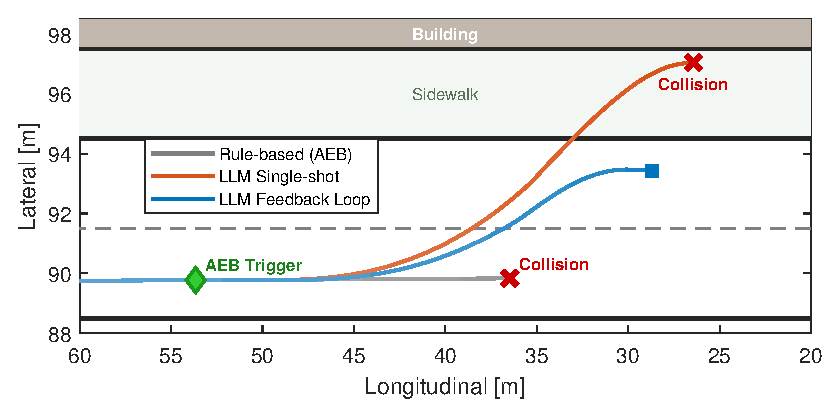
\includegraphics[width=\columnwidth]{Fig_Trajectory.eps}
	\caption{제어 방식별 차량 궤적 비교. Rule-based는 직진 후 보행자와 충돌, Single-shot은 좌측 회피를 시도하나 보도 영역에서 충돌, Feedback Loop는 보행자를 회피하며 차로 내 제어를 유지하였다.}
	\label{fig_trajectory}
\end{figure}

\begin{figure}[tbp!]
	\centering
	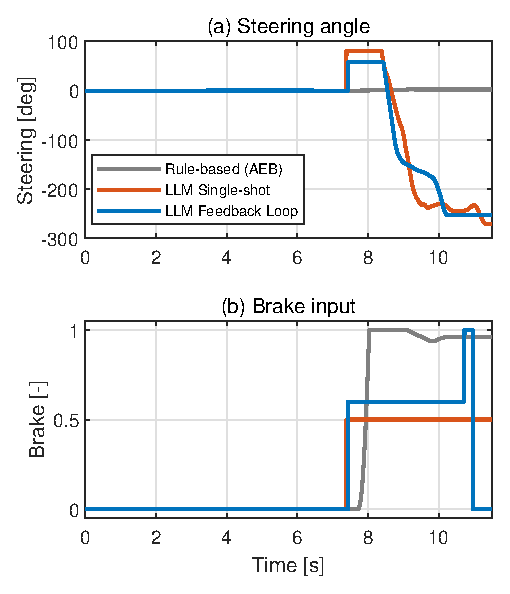
\includegraphics[width=\columnwidth]{Fig_ControlInput.eps}
	\caption{제어 방식별 조향각 및 제동 입력 비교. (a) Rule-based는 조향이 거의 없으며, Single-shot과 Feedback Loop는 LLM이 생성한 조향 명령이 반영된다. (b) 세 방식 모두 AEB 제동이 작동하며, LLM 방식은 추가 제동 명령을 생성한다.}
	\label{fig_control}
\end{figure}

\begin{figure}[tbp!]
	\centering
	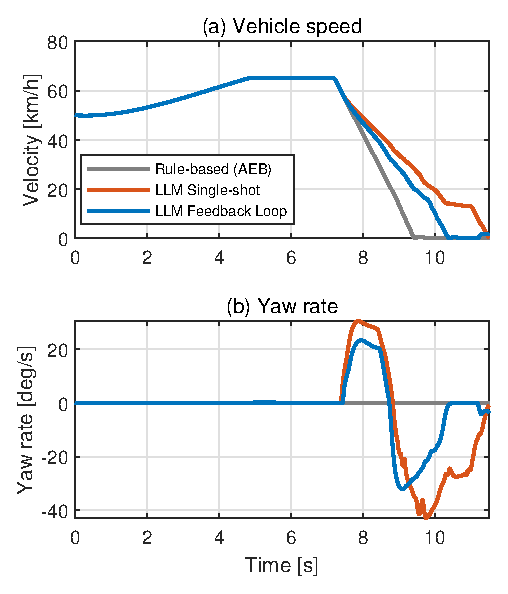
\includegraphics[width=\columnwidth]{Fig_VehicleResponse.eps}
	\caption{제어 방식별 차량 응답 비교. (a) 차량 속도 변화. (b) 요레이트 변화로, Single-shot에서 과도한 요레이트가 발생하여 차량 안정성이 저하됨을 확인할 수 있다.}
	\label{fig_response}
\end{figure}

Table~\ref{tab_comparison}는 세 가지 제어 방식의 LLM 제어 입력과 결과를 정리한 것이다.

\begin{table}[htbp]
\centering
\caption{Comparison of control methods.}
\label{tab_comparison}
\resizebox{\columnwidth}{!}{%
\begin{tabular}{@{}lccc@{}}
\hline
 & Rule & Single & Feedback \\
 & -based & -shot & Loop \\
\hline
제동 입력         & AEB only & 0.5 & 0.6 \\
조향 입력 (rad)   & ---      & 1.4 & 1.0 \\
충돌 여부         & 보행자 충돌 & 건물 충돌 & 회피 성공 \\
\hline
\end{tabular}%
}
\end{table}

Single-shot에서는 LLM이 상황을 올바르게 인식하고 제동과 조향의 복합 회피를 시도하였으나, 1회 판단만으로는 조향량의 적절성을 사전에 검증할 수 없어 과조향이 발생하였다. 반면 Feedback Loop에서는 1차 실행 결과를 LLM이 직접 분석하고, ``조향각이 너무 컸고 차량이 과도하게 이탈하였다''는 판단 하에 제동력 증가와 조향각 감소라는 구체적인 보정 전략을 제시하였다. 이러한 자기 보정(self-correction) 능력은 기존 규칙 기반 방식에서는 구현하기 어려운 LLM 활용의 유의미한 특징이다.

Figure~\ref{fig_trajectory}의 궤적에서 확인할 수 있듯이, Rule-based 방식은 직진 후 보행자와 충돌하였고, Single-shot 방식은 좌측 회피를 시도하였으나 과도한 조향으로 보도 영역에서 충돌하였다. Feedback Loop 방식은 이전 판단을 보정하여 보행자를 회피하면서도 차로 내 제어를 유지하였다. Figure~\ref{fig_response}(b)의 요레이트에서 Single-shot의 과도한 차량 회전이 확인되며, 이는 Figure~\ref{fig_control}(a)의 과조향 입력에 기인한다.


\subsection{논의}
\label{sec:discussion}

본 시스템의 핵심 설계인 트리거 기반 일시정지 전략은 LLM의 응답 지연(수 초)이 차량 제어의 안전성에 영향을 미치지 않도록 한다. 이는 실시간 제어가 요구되는 실차 환경과 달리, 시뮬레이션 환경에서는 시간 흐름을 제어할 수 있다는 특성을 활용한 것이다.

실험 결과에서 주목할 점은 Feedback Loop의 LLM이 단순히 새로운 명령을 생성하는 것이 아니라, 이전 판단의 실패 원인을 자연어로 분석하고 구체적인 수치 보정 근거를 제시한다는 것이다. 이는 LLM의 추론 능력이 제어 파라미터 튜닝에 활용될 수 있음을 시사한다.

다만, Feedback Loop는 LLM을 반복 호출하므로 총 응답 시간이 증가하며, 시뮬레이션 일시정지 시간이 길어지는 트레이드오프가 존재한다. 또한 현재 구조에서는 피드백 루프의 반복 횟수에 대한 종료 조건이 명시적으로 정의되어 있지 않으며, 이는 향후 자동 수렴 판단 메커니즘의 도입을 통해 개선할 수 있다.


%% ============================================================
%% SECTION 5: CONCLUSION (~0.5p)
%% ============================================================
\section{결론}
\label{sec:conclusion}

본 연구는 LLM 에이전트를 활용한 CarMaker 자율주행 시뮬레이션 판단 시스템을 제안하였다. 트리거 기반 제어 루프와 통합 명령 포맷을 통해 LLM의 자연어 추론 능력을 차량 제어에 연결하였으며, 도심 보행자 긴급 회피 시나리오에서 Rule-based, LLM Single-shot, LLM Feedback Loop의 세 가지 방식을 비교한 결과, Feedback Loop 방식에서 LLM이 이전 판단의 실패 원인을 스스로 분석하고 제어 파라미터를 보정하는 자기 보정의 가능성을 보였다. 향후 연구에서는 다양한 자율주행 시나리오로의 검증 확대, 다중 LLM 비교를 통한 최적 모델 선정, 그리고 명령 체계의 범용화를 통해 시뮬레이션 기반 자율주행 의사결정 연구의 확장을 수행할 계획이다.


\section*{사사}
% TODO: 과제 정보
This work was supported by TODO.


\bibliographystyle{elsarticle-num}
\bibliography{ref}

\end{document}

\endinput
